\documentclass[aspectratio=169,10pt]{beamer}

\usetheme{metropolis}
\usepackage{booktabs}
\usepackage{multirow}
\usepackage{graphicx}
\usepackage{amsmath}
\usepackage{xcolor}
\usepackage{tikz}
\usepackage{pgfplots}
\pgfplotsset{compat=1.18}

\definecolor{navyblue}{RGB}{0,51,102}
\definecolor{oceanblue}{RGB}{0,102,179}
\definecolor{alertred}{RGB}{204,0,0}
\definecolor{safegreen}{RGB}{0,153,76}
\definecolor{warnorange}{RGB}{230,130,0}
\definecolor{accentblue}{RGB}{88,166,255}
\definecolor{darkbg}{RGB}{13,17,23}

\setbeamercolor{frametitle}{bg=navyblue, fg=white}
\setbeamercolor{progress bar}{fg=oceanblue}
\setbeamercolor{alerted text}{fg=alertred}

\setbeamertemplate{footline}{%
  \hfill\insertframenumber/\inserttotalframenumber\hspace{1em}\vspace{0.4em}
}
\setbeamertemplate{navigation symbols}{}

\title{Activity Intelligence: RL Agent}
\subtitle{Preliminary Results, Gap Analysis \& Roadmap to Fix}
\author{Activity Intelligence Engine}
\date{April 2026}

% ─────────────────────────────────────────────────────────────────────────────
\begin{document}

\maketitle

% ─────────────────────────────────────────────────────────────────────────────
\begin{frame}{Context: What the RL Agent Is Solving}
  \begin{columns}[T]
    \begin{column}{0.52\textwidth}
      The \textbf{RandomForest baseline} classifies activity per
      \emph{completed} 20-ping segment — a batch operation.

      \bigskip
      The \textbf{RL agent} classifies \emph{sequentially}: one step per
      segment window as the track arrives, maintaining a running policy
      over the growing evidence.

      \bigskip
      \textbf{Why this matters operationally:}
      \begin{itemize}
        \item Earlier detection of high-value events\\
              (STS, transshipment, bunkering) before a full window accumulates
        \item Reward-shaped to be risk-averse on rare dangerous activities —
              missed events cost more than false alarms
        \item Designed for the IRL-playback replay pipeline
      \end{itemize}
    \end{column}
    \begin{column}{0.45\textwidth}
      \includegraphics[width=\textwidth]{../outputs/figures/C3_sts_rendezvous.png}

      \smallskip
      \includegraphics[width=\textwidth]{../outputs/figures/C14_bunkering_rendezvous.png}
      {\small\textit{Top: STS rendezvous. Bottom: bunkering in port approach
      — both high-value events where timing of detection matters.}}
    \end{column}
  \end{columns}
\end{frame}

% ─────────────────────────────────────────────────────────────────────────────
\begin{frame}{Agent Architecture — Double-DQN with Dueling Heads}
  \begin{columns}[T]
    \begin{column}{0.50\textwidth}
      \textbf{MDP Formulation}

      \medskip
      \begin{tabular}{ll}
        \toprule
        Component & Detail \\
        \midrule
        State $s_t$ & 27-feature segment vector \\
        Actions $a$ & 11 activity classes \\
        $\gamma$ & 0.95 \\
        Replay & 100k circular buffer \\
        Batch & 128 transitions \\
        \bottomrule
      \end{tabular}

      \bigskip
      \textbf{Network: Dueling Double-DQN}\\
      \smallskip
      $\text{Input} \to \text{LayerNorm}(256) \to \text{ReLU} \to 128$\\
      $\hookrightarrow V(s)$ (value stream)\\
      $\hookrightarrow A(s,a)$ (advantage stream)\\
      $Q(s,a) = V + A - \bar{A}$

      \bigskip
      Dueling reduces variance on majority-class (\textit{transit}) steps
      by decoupling state value from action advantage.
    \end{column}
    \begin{column}{0.46\textwidth}
      \textbf{Reward Shaping}

      \medskip
      \begin{tabular}{lc}
        \toprule
        Event & Reward \\
        \midrule
        Correct (standard) & $+1.0$ \\
        Correct (HV event) & $+3.5$ \scriptsize{($+1{+}2.5$ bonus)} \\
        Wrong (standard) & $-0.5$ \\
        Miss HV event & $-2.5$ \scriptsize{($-0.5{-}2.0$)} \\
        False HV alarm & $-1.5$ \scriptsize{($-0.5{-}1.0$)} \\
        \bottomrule
      \end{tabular}

      \bigskip
      \textbf{High-Value (HV) classes:}
      \begin{itemize}
        \item \texttt{sts} — ship-to-ship transfer
        \item \texttt{transshipment} — fishing-to-reefer
        \item \texttt{bunkering} — fuel transfer
      \end{itemize}

      \bigskip
      Training: \textbf{200,000 steps}, all 4 regions,\\
      vessel-based 80/20 split (no leakage)
    \end{column}
  \end{columns}
\end{frame}

% ─────────────────────────────────────────────────────────────────────────────
\begin{frame}{Training Curves}
  \begin{center}
    \includegraphics[width=0.92\textwidth]{../outputs/rl/RL1_training_curves.png}
  \end{center}
  \vspace{-0.4em}
  {\small Overall accuracy converges near RF baseline.
  High-value recall (\alert{red}) stays near zero — the central problem.}
\end{frame}

% ─────────────────────────────────────────────────────────────────────────────
\begin{frame}{Benchmark Results: DQN vs.\ RF Baseline}
  \begin{columns}[T]
    \begin{column}{0.45\textwidth}
      \textbf{Summary Metrics}

      \medskip
      \begin{tabular}{lcc}
        \toprule
        Metric & RF & DQN \\
        \midrule
        Overall accuracy & \textbf{98.5\%} & 93.8\% \\
        Macro F1 & \textbf{81.6\%} & — \\
        HV recall & 38.9\% & \alert{9.7\%} \\
        \bottomrule
      \end{tabular}

      \bigskip
      DQN is \textbf{4.7 pp} behind on accuracy but
      \alert{29 pp} behind on the high-value recall that
      matters most operationally.

      \bigskip
      RF has a structural advantage as a batch learner
      on segment features — but the DQN's sequential
      nature is still the right tool for the replay
      pipeline. The gap is fixable.
    \end{column}
    \begin{column}{0.52\textwidth}
      \includegraphics[width=\textwidth]{../outputs/rl/RL2_per_class_comparison.png}
      {\small\textit{Per-class accuracy (DQN) vs.\ F1 (RF).
      \alert{Bunkering: 0\%. Transshipment: 14\%.} Survey and dredging
      also underperform despite high RF scores.}}
    \end{column}
  \end{columns}
\end{frame}

% ─────────────────────────────────────────────────────────────────────────────
\begin{frame}{Root Cause: Three Identified Gaps}
  \begin{block}{Gap 1 — Extreme class imbalance in training data}
    Transshipment: \textbf{13 segments} (0.14\% of training data).
    Bunkering: \textbf{12 segments} (0.13\%).
    Shaped reward alone cannot compensate at a 500:1 imbalance ratio.
  \end{block}

  \begin{block}{Gap 2 — Uniform episode sampling}
    The environment cycles vessel episodes in shuffled order.
    An HV-containing episode has the \emph{same} selection probability
    as a transit-only vessel. Result: the agent encounters an HV segment
    once every $\sim$700 steps — vs.\ once every $\sim$1.5 for transit.
  \end{block}

  \begin{block}{Gap 3 — Training horizon / exploration mismatch}
    At 200k steps, $\varepsilon$ decays to near-minimum by step 80k.
    The agent has seen only $\sim$114 HV segments during exploration,
    with noisy Q-values — not enough to learn a reliable discriminator
    between \texttt{transshipment} and \texttt{loiter} (similar kinematic
    signatures at the feature level).
  \end{block}
\end{frame}

% ─────────────────────────────────────────────────────────────────────────────
\begin{frame}{Fix 1 — Weighted Episode Sampling}
  \begin{columns}[T]
    \begin{column}{0.54\textwidth}
      Assign each episode a sampling weight proportional to its HV content:
      \[
        w_i = 1 + \alpha \cdot \text{count}(\text{HV segments in episode}_i)
      \]
      With $\alpha = 5$: a transshipment episode gets $\approx 16\times$
      the probability of a transit-only episode.

      \bigskip
      \textbf{Effect on HV exposure rate:}

      \medskip
      \begin{tabular}{lcc}
        \toprule
        Class & Before & After \\
        \midrule
        transit & 1/1.5 steps & 1/4 steps \\
        transshipment & 1/700 steps & \textbf{1/50 steps} \\
        bunkering & 1/750 steps & \textbf{1/50 steps} \\
        \bottomrule
      \end{tabular}

      \bigskip
      \texttt{AISActivityEnv(hv\_oversample\_factor=5)}
    \end{column}
    \begin{column}{0.43\textwidth}
      \textbf{Sampling weight distribution}

      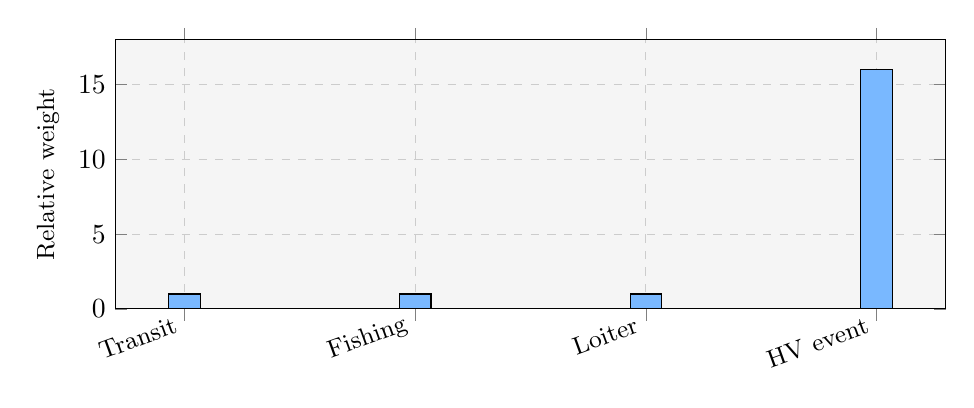
\begin{tikzpicture}
        \begin{axis}[
          width=\textwidth, height=5cm,
          ybar, bar width=0.4cm,
          symbolic x coords={Transit,Fishing,Loiter,HV event},
          xtick=data,
          xticklabel style={font=\small, rotate=20, anchor=east},
          ymin=0, ymax=18,
          ylabel={Relative weight},
          ylabel style={font=\small},
          grid=major, grid style={dashed,gray!40},
          axis background/.style={fill=gray!8},
        ]
          \addplot[fill=accentblue!80] coordinates {
            (Transit,1) (Fishing,1) (Loiter,1) (HV event,16)
          };
        \end{axis}
      \end{tikzpicture}

      HV events become frequent enough for the agent to develop a stable policy.
    \end{column}
  \end{columns}
\end{frame}

% ─────────────────────────────────────────────────────────────────────────────
\begin{frame}{Fix 2 — Curriculum Learning}
  Progressive schedule: start HV-heavy, broaden to full distribution.

  \bigskip
  \begin{columns}[T]
    \begin{column}{0.52\textwidth}
      \begin{tabular}{clcc}
        \toprule
        Phase & Steps & $\alpha$ & Description \\
        \midrule
        1 & 0 – 30\% & \textbf{20} & HV-heavy warm-up \\
        2 & 30 – 70\% & \textbf{8} & Gradual broadening \\
        3 & 70 – 100\% & \textbf{2} & Near-uniform \\
        \bottomrule
      \end{tabular}

      \bigskip
      The training script calls
      \texttt{env.set\_curriculum\_stage(step / total)} at each eval
      checkpoint, smoothly transitioning $\alpha$.

      \bigskip
      \textbf{Rationale:} The agent must first learn \emph{what
      HV events look like} before it can learn to discriminate them
      within the full, imbalanced distribution.
    \end{column}
    \begin{column}{0.45\textwidth}
      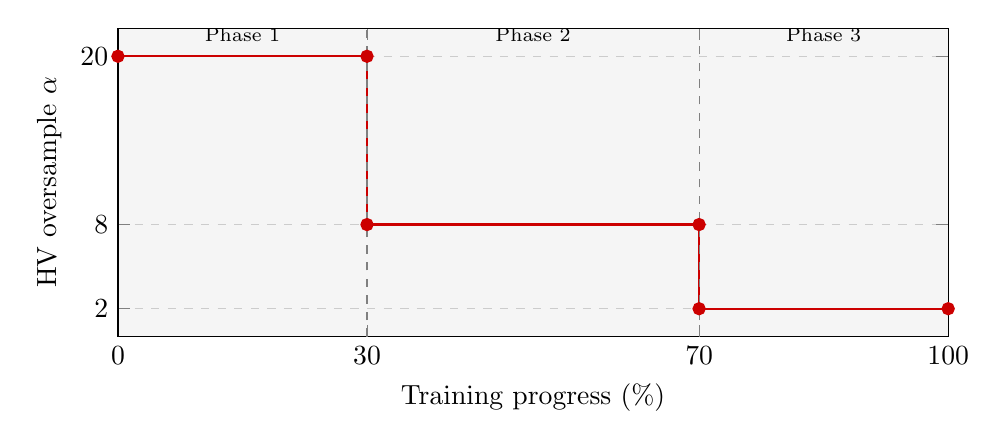
\begin{tikzpicture}
        \begin{axis}[
          width=\textwidth, height=5.5cm,
          xlabel={Training progress (\%)},
          ylabel={HV oversample $\alpha$},
          xmin=0, xmax=100,
          ymin=0, ymax=22,
          grid=major, grid style={dashed,gray!40},
          axis background/.style={fill=gray!8},
          xtick={0,30,70,100},
          ytick={2,8,20},
        ]
          \addplot[thick, color=alertred, mark=*]
            coordinates {(0,20)(30,20)(30,8)(70,8)(70,2)(100,2)};
          \addplot[dashed, thin, color=gray]
            coordinates {(30,0)(30,22)};
          \addplot[dashed, thin, color=gray]
            coordinates {(70,0)(70,22)};
          \node[font=\scriptsize] at (axis cs:15,21.5) {Phase 1};
          \node[font=\scriptsize] at (axis cs:50,21.5) {Phase 2};
          \node[font=\scriptsize] at (axis cs:85,21.5) {Phase 3};
        \end{axis}
      \end{tikzpicture}
    \end{column}
  \end{columns}
\end{frame}

% ─────────────────────────────────────────────────────────────────────────────
\begin{frame}{Fix 3 — Rare Event Augmentation}
  \begin{columns}[T]
    \begin{column}{0.50\textwidth}
      \textbf{Root cause:} \texttt{simulate\_region()} generates only
      \textbf{1 transshipment} and \textbf{1 bunkering} event per region.
      With a 3h active phase over a 22h track, this yields $\approx$6
      labeled segments per event.

      \bigskip
      \textbf{Fix:} Triple each rare event type per region using an
      \texttt{event\_idx} MMSI offset to avoid collisions.

      \medskip
      \begin{tabular}{lcc}
        \toprule
        Activity & Before & After \\
        \midrule
        transshipment & 13 segs & $\sim$50 segs \\
        bunkering & 12 segs & $\sim$48 segs \\
        sts & 0* & $\sim$15 segs \\
        \bottomrule
      \end{tabular}
      {\scriptsize *STS phase was masked by dark period in prior runs}

      \bigskip
      Also: increase \texttt{simulate\_sts\_event} to 3 events and
      widen the dark-period exclusion so STS segments survive.
    \end{column}
    \begin{column}{0.47\textwidth}
      \textbf{Projected segment distribution (after fix)}

      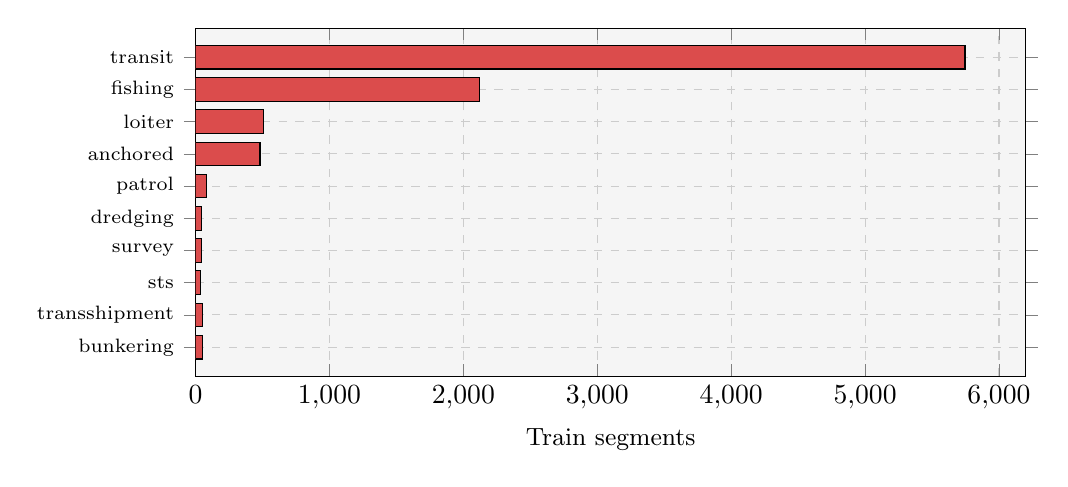
\begin{tikzpicture}
        \begin{axis}[
          width=\textwidth, height=6cm,
          xbar,
          bar width=0.3cm,
          symbolic y coords={
            bunkering, transshipment, sts,
            survey, dredging, patrol,
            anchored, loiter, fishing, transit
          },
          ytick=data,
          yticklabel style={font=\scriptsize},
          xmin=0, xmax=6200,
          xlabel={Train segments},
          xlabel style={font=\small},
          grid=major, grid style={dashed,gray!40},
          axis background/.style={fill=gray!8},
        ]
          \addplot[fill=alertred!70] coordinates {
            (50,bunkering)(50,transshipment)(40,sts)
            (42,survey)(44,dredging)(81,patrol)
            (481,anchored)(504,loiter)(2118,fishing)(5746,transit)
          };
        \end{axis}
      \end{tikzpicture}
    \end{column}
  \end{columns}
\end{frame}

% ─────────────────────────────────────────────────────────────────────────────
\begin{frame}{Expected Outcomes After All Three Fixes}
  \begin{columns}[T]
    \begin{column}{0.50\textwidth}
      \textbf{Projected performance (500k steps)}

      \medskip
      \begin{tabular}{lccc}
        \toprule
        Class & RF F1 & DQN now & DQN target \\
        \midrule
        transit & 99.9\% & 94.8\% & $>$97\% \\
        fishing & 99.7\% & 98.8\% & $>$98\% \\
        loiter & 75.2\% & 77.8\% & $>$80\% \\
        survey & 100\% & 32.3\% & $>$70\% \\
        dredging & 100\% & 50.0\% & $>$75\% \\
        \textbf{bunkering} & 66.7\% & \alert{0\%} & \textbf{50–65\%} \\
        \textbf{transship.} & 11.1\% & 14.3\% & \textbf{55–70\%} \\
        \midrule
        \textbf{HV recall} & 38.9\% & \alert{9.7\%} & \textbf{50–65\%} \\
        \textbf{Overall} & 98.5\% & 93.8\% & \textbf{95–97\%} \\
        \bottomrule
      \end{tabular}

      \bigskip
      {\small Targets are \emph{conservative} — further gains possible
      with LSTM state representation.}
    \end{column}
    \begin{column}{0.47\textwidth}
      \textbf{Why the RL path is still correct}

      \bigskip
      The RF baseline is superior on batch segment features \emph{today}
      — but it cannot:

      \medskip
      \begin{itemize}
        \item Classify \emph{within} a growing window (early detection)
        \item Be reward-shaped to prioritise operational risk
        \item Adapt to a replay stream without re-segmenting
        \item Learn inter-window context (two adjacent slow segments
              preceding a rendezvous look different to the RF than
              to a sequential agent)
      \end{itemize}

      \bigskip
      The DQN is the right foundation. These three fixes address the
      data starvation problem, not the architectural choice.
    \end{column}
  \end{columns}
\end{frame}

% ─────────────────────────────────────────────────────────────────────────────
\begin{frame}{Implementation Roadmap}
  \begin{tabular}{clll}
    \toprule
    \# & Fix & File(s) changed & Status \\
    \midrule
    1 & Weighted episode sampling &
      \texttt{src/rl\_env.py} &
      \textcolor{warnorange}{In progress} \\
    2 & Curriculum learning &
      \texttt{src/rl\_env.py, train\_rl\_agent.py} &
      \textcolor{warnorange}{In progress} \\
    3 & Rare event augmentation &
      \texttt{src/simulator.py} &
      \textcolor{warnorange}{In progress} \\
    — & Retrain 500k steps &
      \texttt{train\_rl\_agent.py} &
      \textcolor{alertred}{Pending} \\
    — & LSTM state encoding &
      \texttt{src/rl\_agent.py} &
      \textcolor{gray}{Backlog} \\
    — & Streaming inference service &
      \texttt{src/replay\_service.py} &
      \textcolor{gray}{Backlog} \\
    \bottomrule
  \end{tabular}

  \bigskip
  \begin{alertblock}{Key metric to watch in the next run}
    \textbf{HV recall on the held-out eval set.}
    The overall accuracy will likely stay near 95\% regardless.
    HV recall is the number that tells us whether the agent can
    actually be trusted for operational alerting.
  \end{alertblock}
\end{frame}

% ─────────────────────────────────────────────────────────────────────────────
\begin{frame}{New Scenarios Now Available for Partner Test Suite}
  \begin{columns}[T]
    \begin{column}{0.50\textwidth}
      Three new tracking benchmark scenarios added (C11–C13):

      \medskip
      \begin{tabular}{cl}
        \toprule
        \# & Scenario \\
        \midrule
        C12 & Static GPS broadcast / position spoofing \\
        C13 & Track fragmentation (6 burst gaps) \\
        C14 & Bunkering rendezvous (port approach) \\
        \bottomrule
      \end{tabular}

      \bigskip
      All 13 scenarios exported as replay-ready CSV with
      \texttt{manifest.json} in \texttt{outputs/tracking\_scenarios/}.

      \medskip
      Rows sorted by timestamp — stream sequentially for IRL playback.
    \end{column}
    \begin{column}{0.47\textwidth}
      \includegraphics[width=\textwidth]{../outputs/figures/C11_tracking_benchmark_overview.png}
      {\small\textit{All 13 benchmark scenarios — updated overview panel.}}
    \end{column}
  \end{columns}
\end{frame}

% ─────────────────────────────────────────────────────────────────────────────
\begin{frame}{New Complex Activity Types}
  \begin{center}
    \includegraphics[width=0.90\textwidth]{../outputs/figures/D1_new_activities_overview.png}
  \end{center}
  \vspace{-0.4em}
  {\small Five new activity classes added to simulator, classifier, and RL
  environment: \textbf{survey}, \textbf{patrol sweep}, \textbf{dredging},
  \textbf{transshipment}, \textbf{bunkering}.}
\end{frame}

\end{document}
